\documentclass[12pt]{article}
\usepackage{fullpage}
\usepackage[utf8]{inputenc}
\usepackage{listings}
\usepackage{color} %needed by the ``\definecolor''

\usepackage{framed} %needed by the ``shaded'' environment which is responsible for the background color of the verbatim text block
\usepackage{verbatim} %needed by the ``\verbatim'' command which is part of the environment responsible for the background color of the verbatim text block

\usepackage{graphicx}
\usepackage{hyperref} %the hyperref package has to be used after all other packages have already been used

%%My definitions {

%%code in-line text
\newcommand{\code}[1]
{\definecolor{shadecolor}{rgb}{0.9,0.9,0.9} \shaded \verbatim #1 \endverbatim \endshaded}

%%important stuff
\newcommand{\imp}[1]
{\textbf{#1}}

%%Source code style settings
%%--------------------------
\definecolor{src_color}{rgb}{0.9,0.9,0.9}

\lstset{language=Python, %default language name
	basicstyle=\small, %font size
%	keywordstyle=\color{blue},
%	commentstyle=\color{red},
%	stringstyle=\color{dkgreen}, 
	backgroundcolor=\color{src_color}, %background color
	numbers=left, numberstyle=\tiny, numbersep=5pt, %listing line numbers styles
	breaklines=true, % sets automatic line breaking
	tabsize=4 %each tab character equals to 4 spaces
}

%%My definitions }

\title{Concurrent tree exploration algorithm}
\author{Mateusz Kobos}

\begin{document}

\maketitle

We will present a tree exploring algorithm with concurrent threads or processes traversing the tree.

Main assumption:
\begin{itemize}
	\item moving between nodes and processing them is time-consuming (expensive).
\end{itemize}

This assumption is particularly true in the application domain that is of our interest. In this domain the threads are independent web crawlers which explore tree-like web page document structure.

All of the threads share a common tree structure which corresponds to the tree part that has been explored by the threads.

During the algorithm run new nodes are added to the tree, nodes are never removed from the tree.

Tree exploration in Python-like pseudocode:

\lstset{language=Python}
\lstinputlisting{pseudocode.py}

\begin{figure}[!ht]
	\centering
		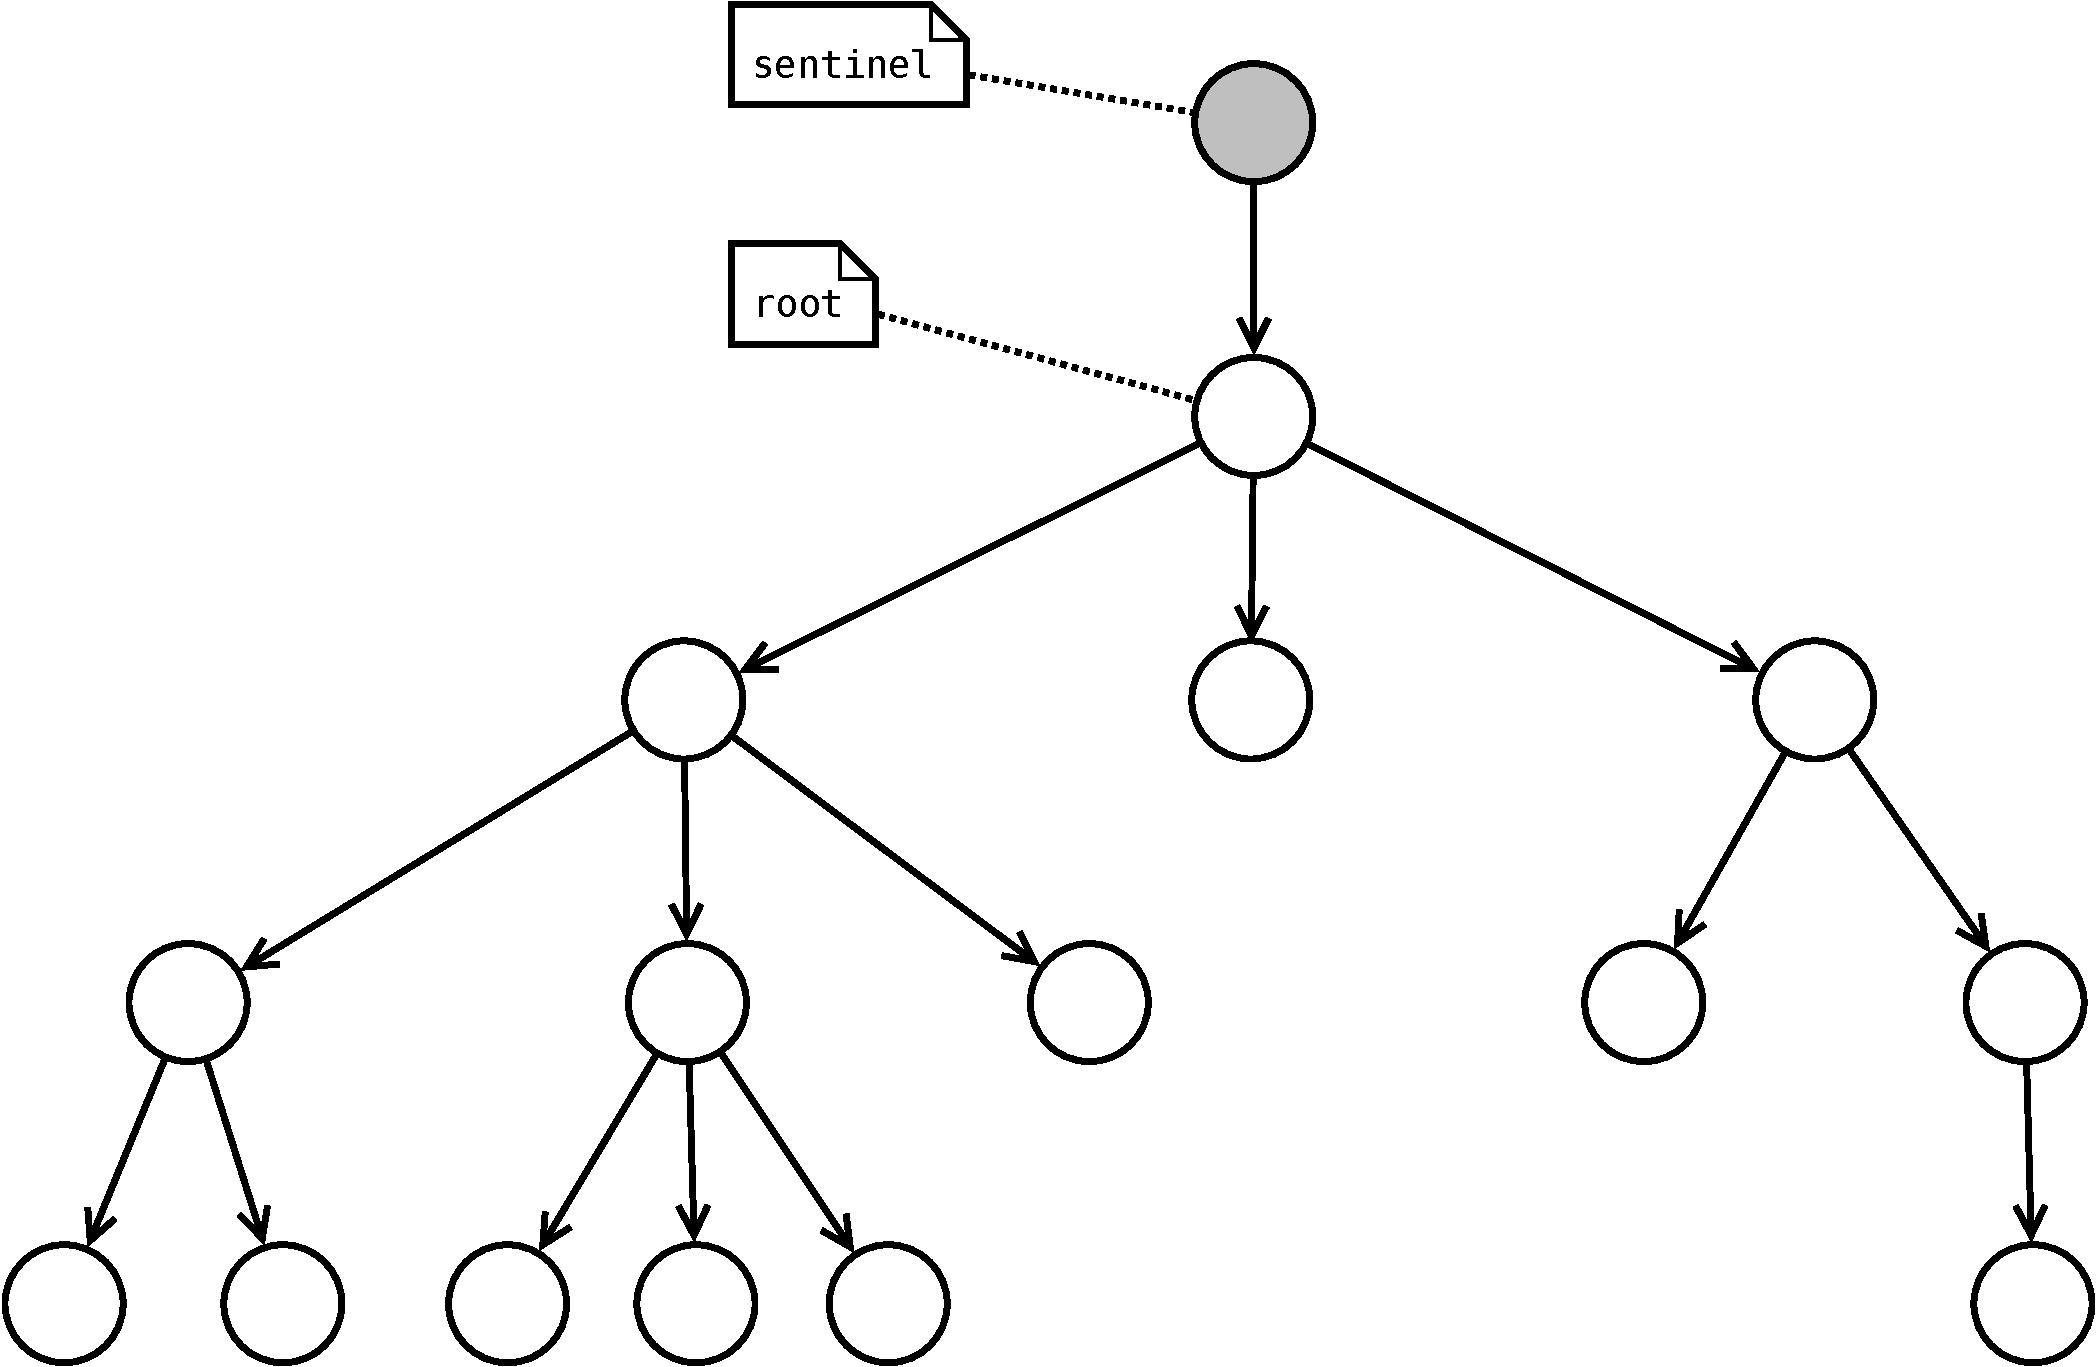
\includegraphics[scale=0.35]{pics/tree.pdf}
	\caption{Traversed tree.}
	\label{fig:tree}
\end{figure}

\begin{figure}[!ht]
	\centering
		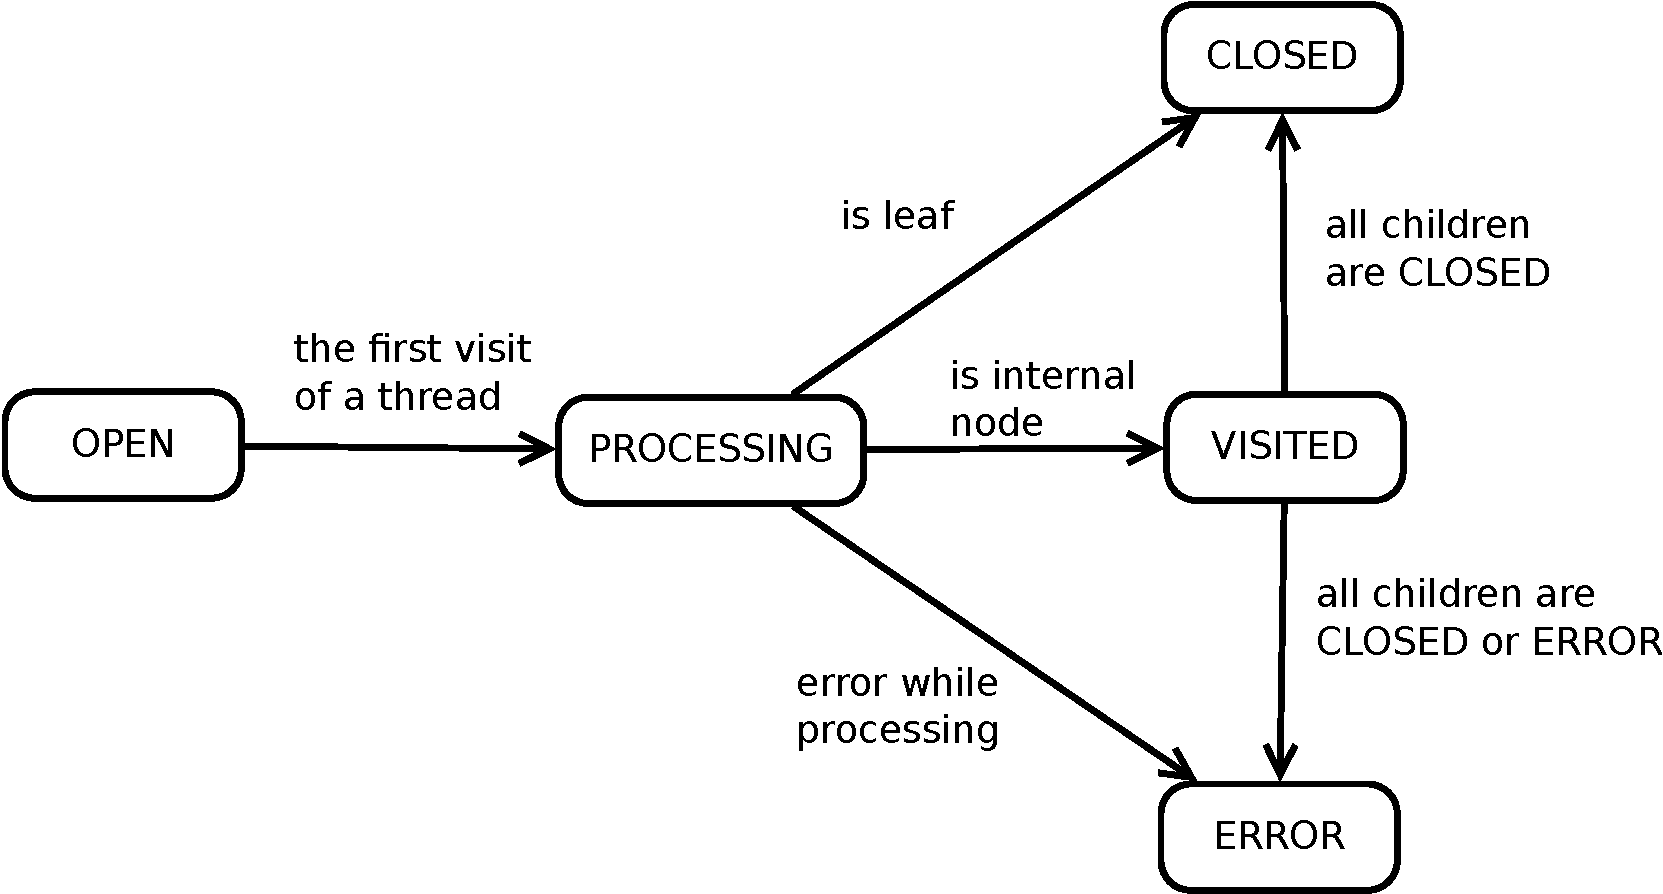
\includegraphics[scale=0.35]{pics/states.pdf}
	\caption{Possible states of a single node and passages between them.}
	\label{fig:states}
\end{figure}

\begin{figure}[!ht]
	\centering
		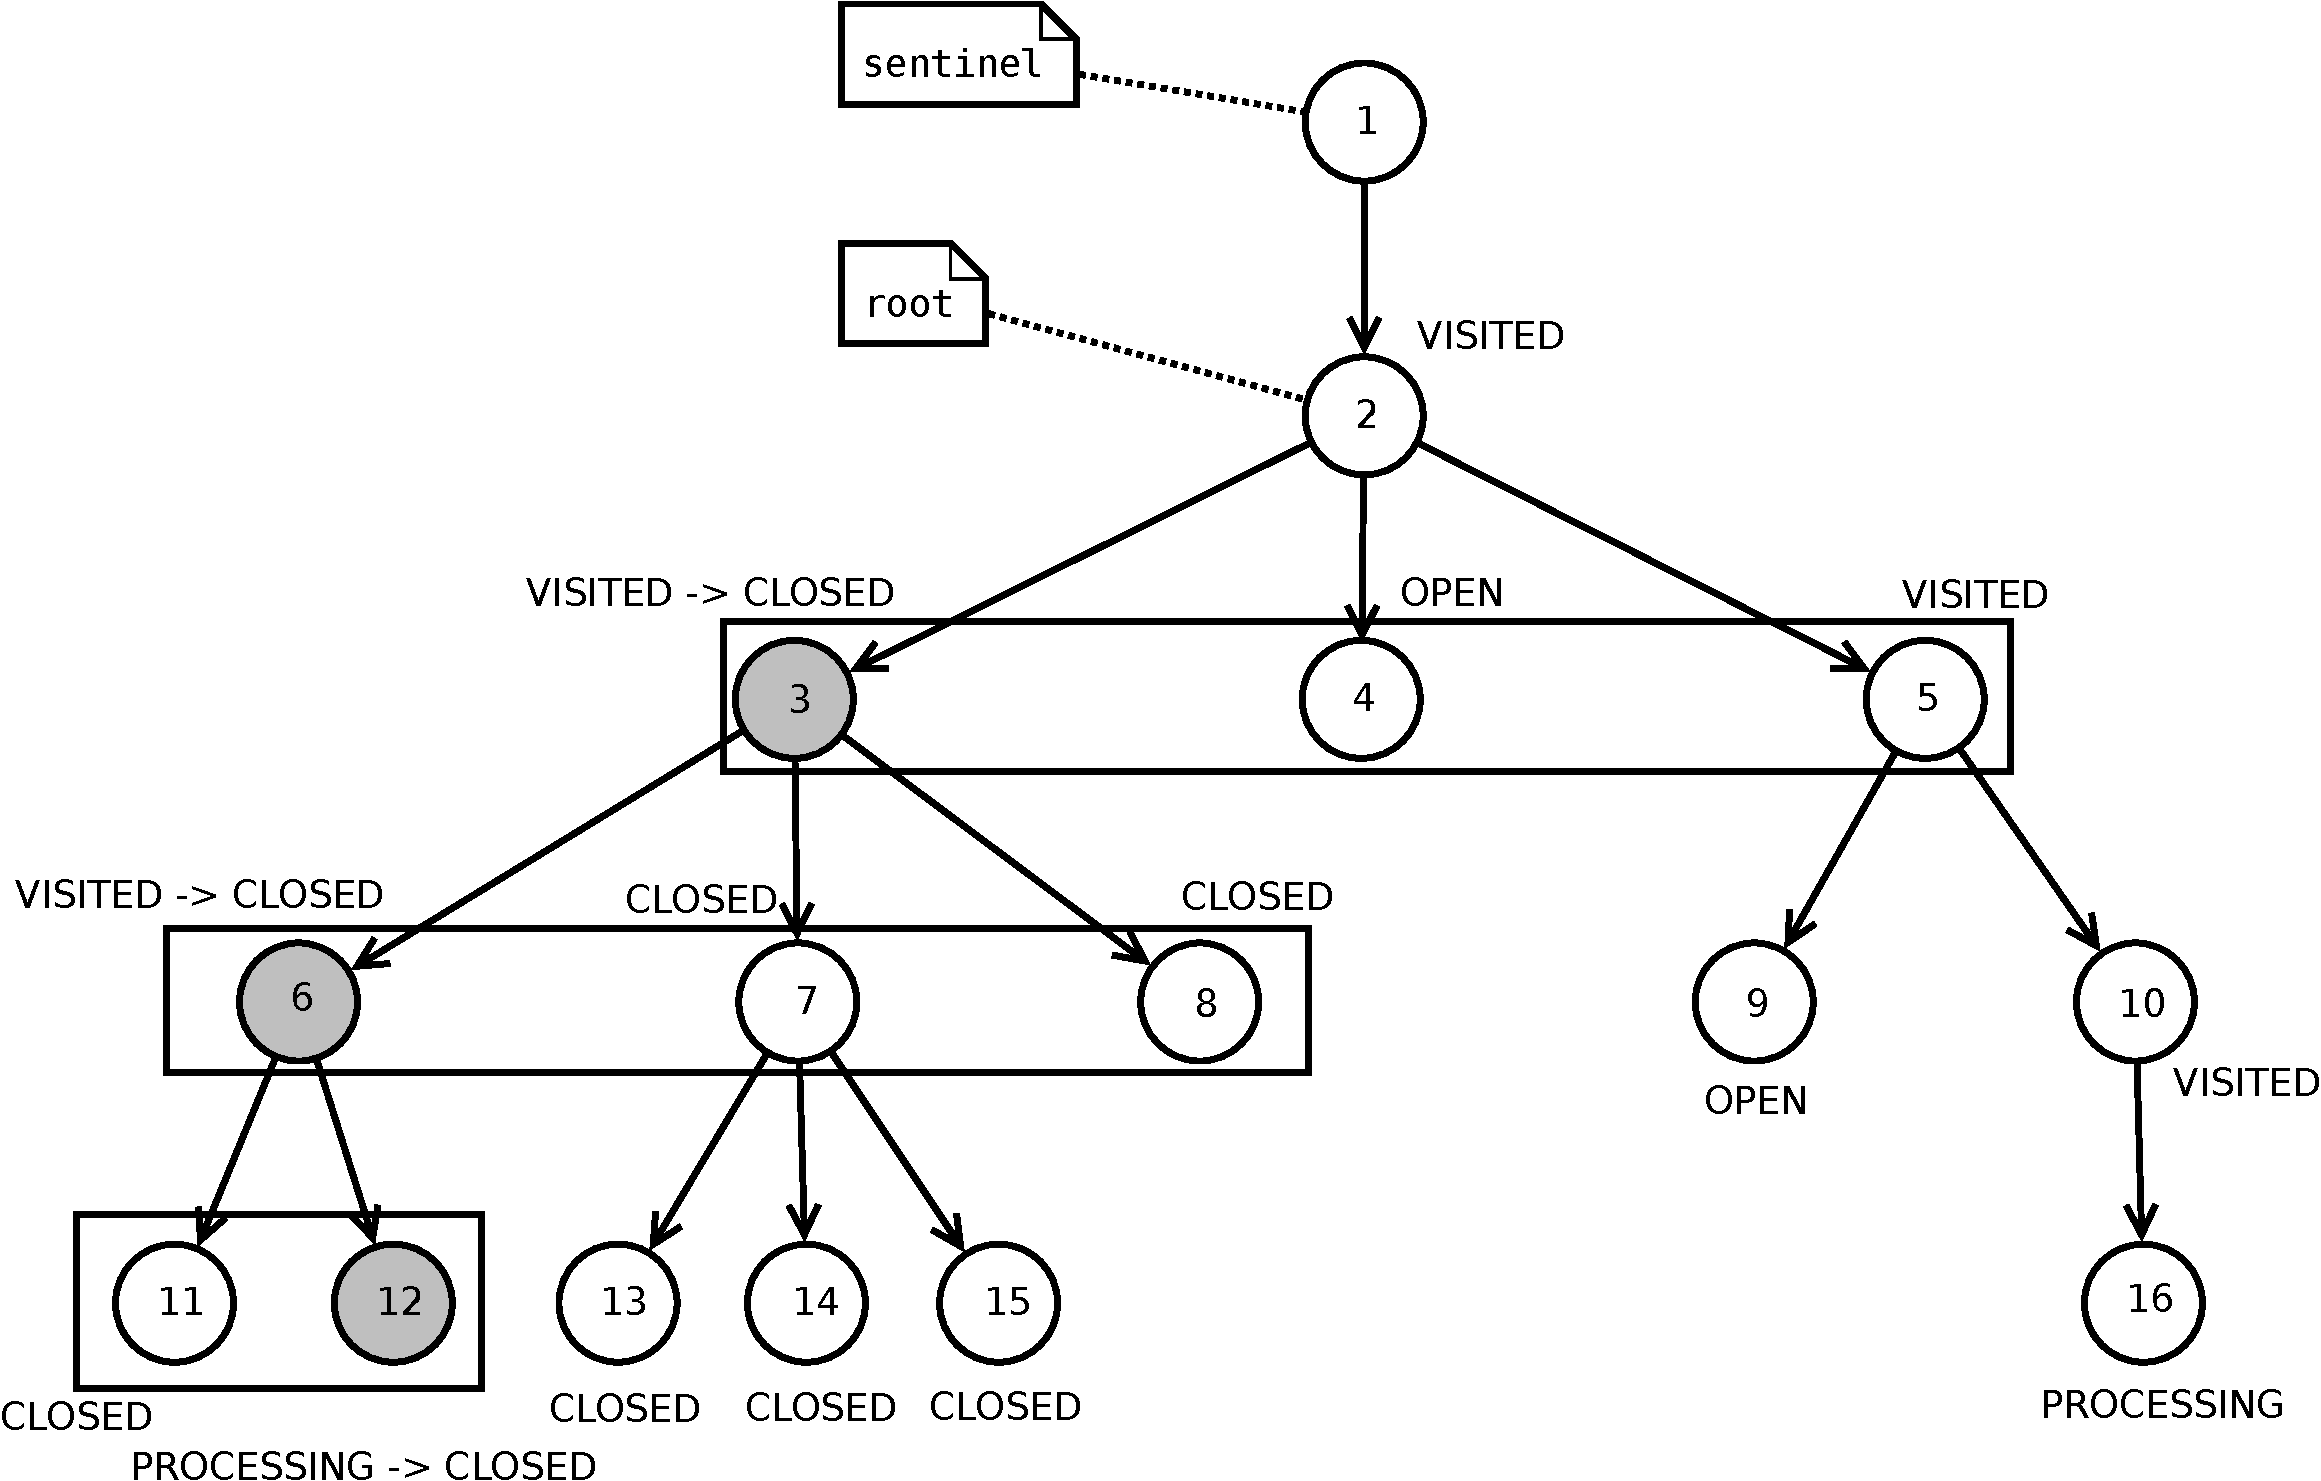
\includegraphics[scale=0.35]{pics/tree-update_upward.pdf}
	\caption{Updating the state of the nodes from the bottom to the top.}
	\label{fig:tree-update_upward}
\end{figure}

\end{document}